%!TEX root = ../../csuthesis_main.tex
\chapter{CORnet-S模型复现与基线分析}

\section{复现流程与实验配置}

\subsection{数据集选型与预处理}

CORnet-S模型是类脑视觉建模中典型的时间递归结构模型,其引入“时间步”(time steps)以模拟视觉皮层多次循环加工过程。为验证该模型在轻量级图像分类任务中的性能表现,并为后续结构改进提供对照基线,本文在 Tiny-ImageNet-200 数据集上对 CORnet-S 进行了完整复现与训练。

Tiny-ImageNet-200是ImageNet的精简版本,包含200个类别,每类有500张训练图像、50张验证图像和50张测试图像,图像尺寸为64×64,数据集总规模约为120,000张。相较于原始 ImageNet(包含1000类,超过120万张图像),Tiny-ImageNet具有体量小、任务完整、结构规范等特点,适合用于原型模型调试与类脑结构验证实验。

\begin{table}[htb]
	\centering
	\caption{Tiny-ImageNet 数据集结构与规模统计表}
	\label{tab:tinyimagenet}
	\begin{tabular}{lllll}
		\hline
		数据划分 & 类别数 & 每类图像数 & 总图像数 & 图像尺寸 \\
		\hline
		训练集(train) & 200 & 500  & 100,000  & 64 × 64 × 3 \\
		验证集(val)   & 200 & 50   & 10,000   & 64 × 64 × 3 \\
		测试集(test)  & 200 & —    & 10,000   & 64 × 64 × 3 \\
		\textbf{合计}   & \textbf{200} & — & \textbf{120,000} & — \\
		\hline
	\end{tabular}
\end{table}

在数据预处理过程中,训练集采用了随机裁剪、随机水平翻转和标准化处理。随即裁剪尺寸保持为$224×224$,标准化处理均值为$[0.485,0.456,0.406]$,标准差为$[0.229,0.224,0.225]$。
验证集和测试集使用统一的中心裁剪策略,并统一缩放到224×224,以保证评估过程的稳定性。所有图像在进入模型前均经过ToTensor( )转换并标准化处理,保持与ImageNet预训练模型输入风格一致。训练与验证数据加载使用PyTorch的ImageFolder接口,分别配置了4个并行数据读取线程,以减少I/O阻塞对训练效率的影响。

\subsection{模型加载与训练细节}

本文使用原始CORnet项目中公开的CORnet-S模型结构代码,并根据论文配置进行参数设定。模型包含四个主要处理模块(V1、V2、V4、IT),其中V2、V4和IT模块均含有时间递归计算,每个时间步均共享权重。模型的decoder部分包含全局平均池化和全连接输出层,为了适配ImageNet分类任务,最终输出维度为1000。

损失函数采用交叉熵损失(CrossEntropyLoss),优化器选择动量梯度下降(SGD),初始学习率设置为0.1,动量系数为0.9,权重衰减系数为$1\times 10^{-4}$。为加快收敛并避免过拟合,采用步长为10的学习率衰减策略(StepLR),每训练10个epoch将学习率缩小10倍。

训练过程共设置43个epoch,batch size为256,与原项目保持一致,使用单张NVIDIA RTX 3090GPU进行加速训练,启用了cuDNN的自动优化模式(torch.backends.cudnn.benchmark = True),以提高卷积计算效率。
模型每个epoch在验证集上进行一次评估,并记录Top-1和Top-5准确率并最终生成results.pkl的文件。训练日志与模型权重定期保存至输出路径,便于恢复训练与后续分析。

\section{性能验证}

\subsection{验证集与测试集Top-1/Top-5准确率对齐}

为验证复现后的CORnet-S模型在Tiny-ImageNet-200数据集上的分类能力,本文对训练过程中的模型性能进行了记录与分析。重点关注模型在验证集与训练集上的Top-1和Top-5准确率变化情况,以及损失函数的收敛趋势。

为更直观地展示模型在不同类别层级的识别能力,Top-1准确率用于衡量模型是否能准确预测图像的主类别标签,而Top-5准确率则反映模型是否将正确类别包含在前5个高置信度预测中。在Tiny-ImageNet这类小样本多类别任务中,Top-5准确率常作为模型泛化能力的重要参考指标。

\begin{figure}[hbt]
	\centering
	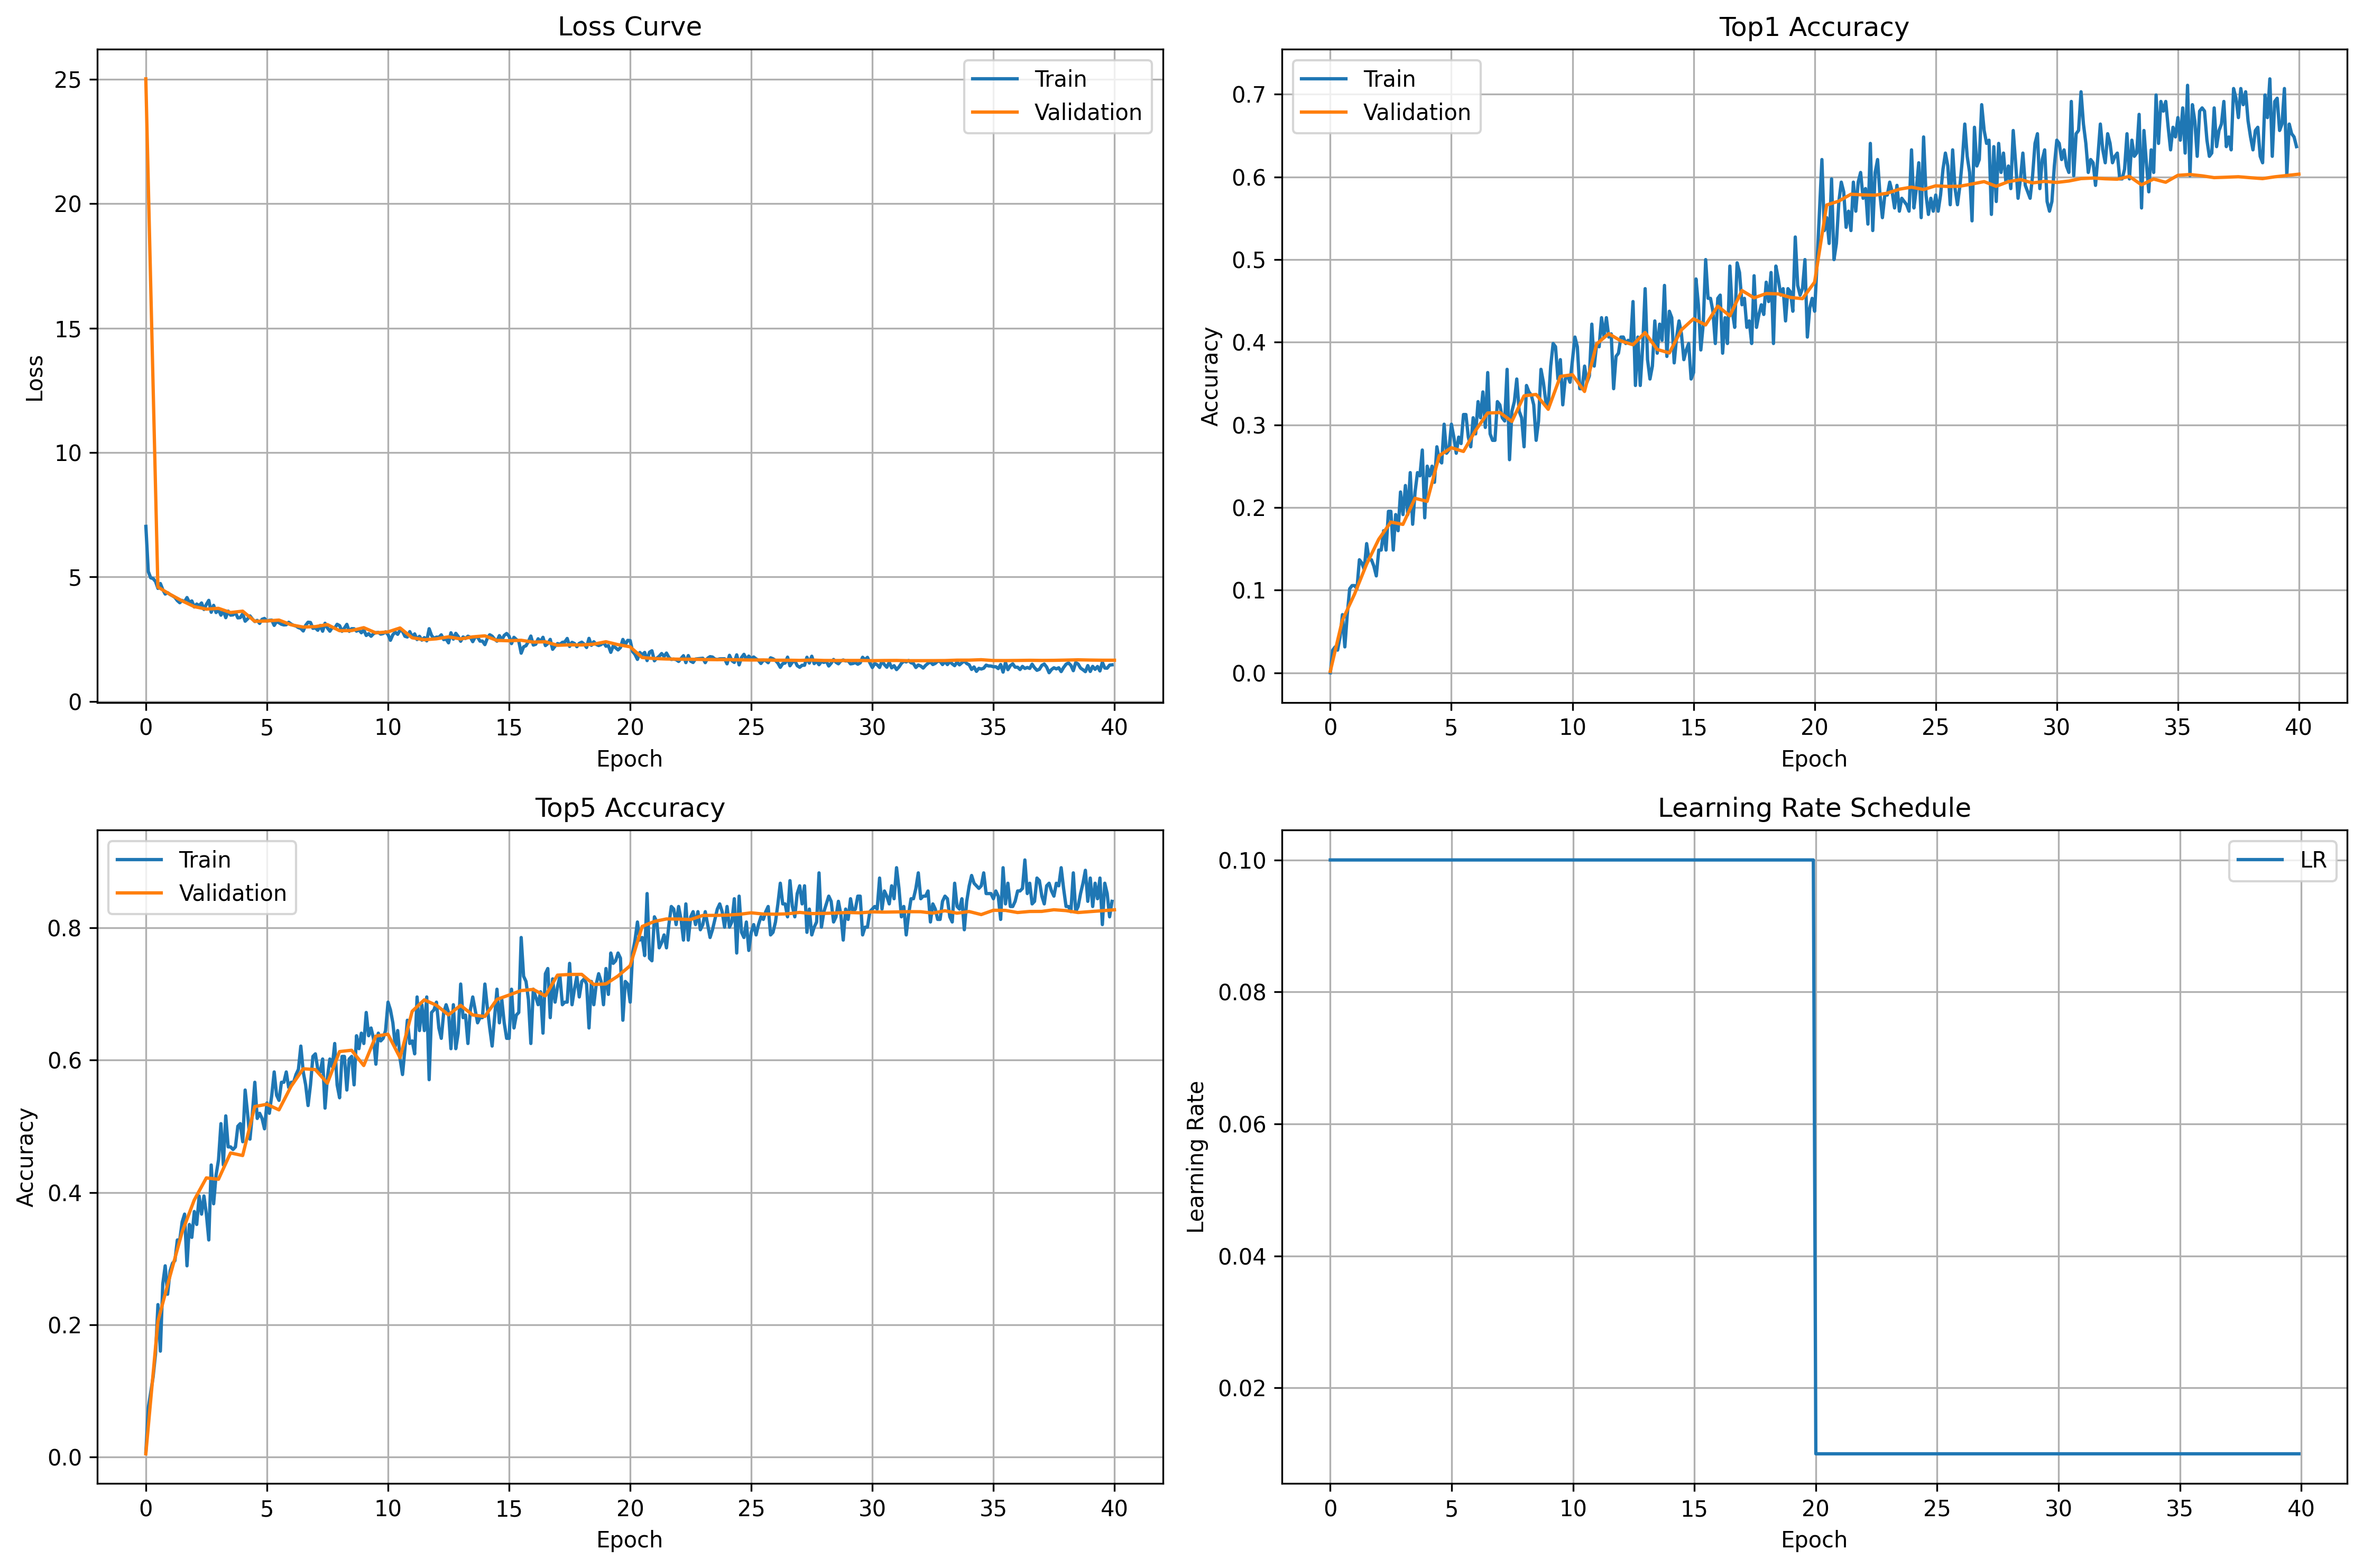
\includegraphics[width=0.8\linewidth]{cornet-s.png}
	\caption{CORnet-S训练数据变化图}
	\label{f.szxt}
\end{figure}

如图\ref{f.szxt}所示,在训练40个epoch后,模型达到其在验证集上的最佳表现。验证结果显示,模型的Top-1准确率为60.34\%,Top-5准确率为82.70\%,对应的交叉熵损失为1.6567。与此同时,模型在训练集上的Top-1准确率为63.67\%,Top-5准确率为83.98\%,训练损失为1.4718。验证集与训练集的准确率差距较小,表明模型在当前配置下未出现明显的过拟合现象,训练过程较为稳定。

\subsection{与原始论文结果对比}

原始的CORnet-S模型由Kubilius等人于2019年在NeurIPS会议中提出,其在ImageNet数据集上的Top-1准确率为74.4\%(Kubilius et al.,2019),在维持较小参数量的前提下,表现出接近ResNet-50的分类性能。同时,该模型在Brain-Score框架下的IT区神经预测得分达到0.604,被视为在准确率与类脑性之间达到较好平衡的代表性架构。

本文在Tiny-ImageNet-200数据集上复现该模型,并使用标准训练配置进行训练与评估,最终在验证集上获得60.34\%的Top-1准确率和82.70\%的Top-5准确率。尽管该结果无法直接与原论文的ImageNet实验对齐,但在样本数量较少、图像尺寸较低的前提下,模型依然展现出稳定的识别能力,说明其结构在小样本多类别任务中同样具有较强适应性。

\begin{table}[htb]
	\centering
	\caption{CORnet-S准确率对比表}
	\label{tab:CORnet-S}
	\begin{tabular}{lllll}
		\hline
		       & 原始CORnet-S & 本文复现的CORnet-S \\
		\hline
		TOP1准确率 & 74.4\% & 60.34\%   \\
		TOP5准确率 & — & 82.70\%    \\
		\hline
	\end{tabular}
\end{table}

需要指出的是,Tiny-ImageNet的难度相较于完整的ImageNet仍有显著差异,类别缩减和图像简化会使模型更容易收敛。因此本实验的结果更多用于结构复现与改进对照,不可与完整 ImageNet 上的结果直接类比。但整体表现仍验证了CORnet-S在轻量级视觉任务中的有效性,也为后续结构优化与注意力机制集成提供了可靠基线。

\section{基线可视化分析}

\subsection{Grad-CAM可视化激活图分析}

Grad-CAM是一种基于梯度的类激活可视化方法,其核心思路是在给定目标类别的前提下,利用该类别在模型输出中的得分对中间特征图的梯度信息进行加权,从而生成一张热力图,直观反映模型在输入图像中“关注”的区域。
在本实验中,选择CORnet-S模型的IT层作为可视化目标层,对验证集中典型图像样本进行激活响应分析。图\ref{f.it_s_act}展示了该模型在IT层的六个典型通道的激活结果。

\begin{figure}[hbt]
	\centering
	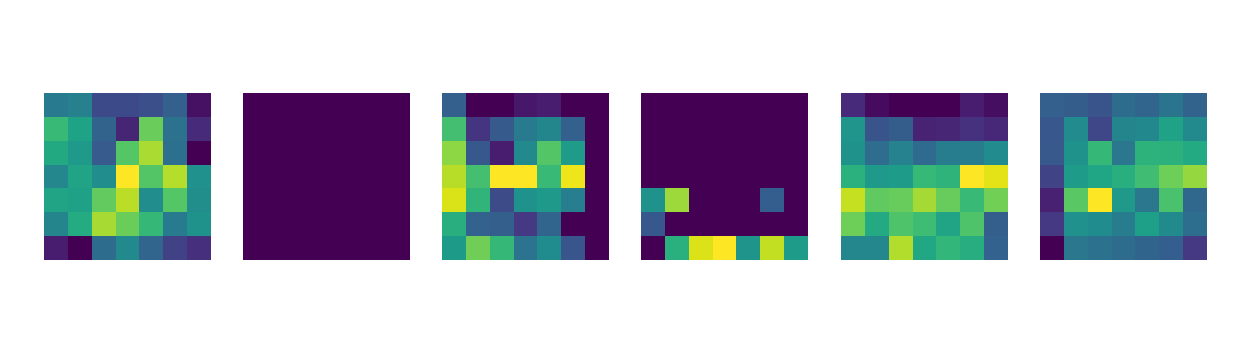
\includegraphics[width=0.8\linewidth]{IT_s_activations.png}
	\caption{CORnet-S模型IT层激活图}
	\label{f.it_s_act}
\end{figure}

观察图像可见,模型在多个通道中对图像主体区域(如摩托车轮廓、前轮等)产生了高响应,说明IT层能够聚焦于具有显著判别力的高阶语义特征。此外,部分通道对图像边缘或背景响应较弱,进一步印证该层在完成判别任务时具备一定的空间注意能力。

\subsection{关键区域关注能力探讨}

为进一步分析CORnet-S模型在不同层级的感知能力,图\ref{f.v1_s_act}至图\ref{f.v4_s_act}分别展示了模型在V1、V2和V4层的激活热力图。

\begin{figure}[hbt]
	\centering
	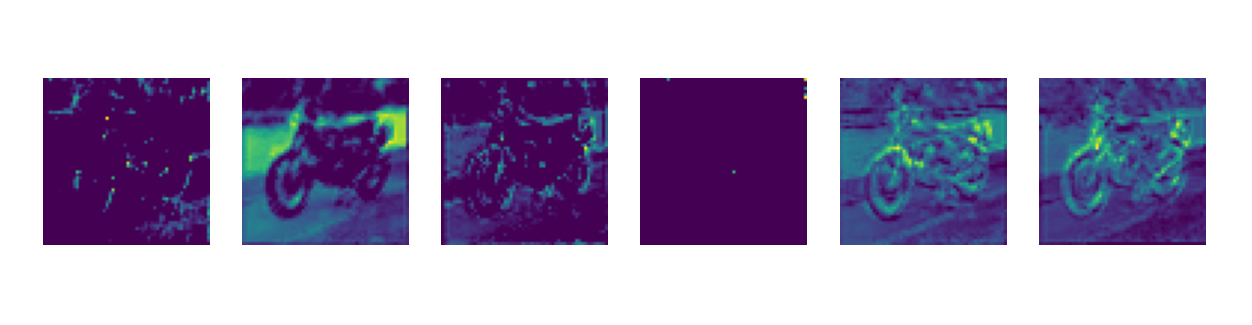
\includegraphics[width=0.8\linewidth]{V1_s_activations.png}
	\caption{CORnet-S模型V1层激活图}
	\label{f.v1_s_act}
\end{figure}

\begin{figure}[hbt]
	\centering
	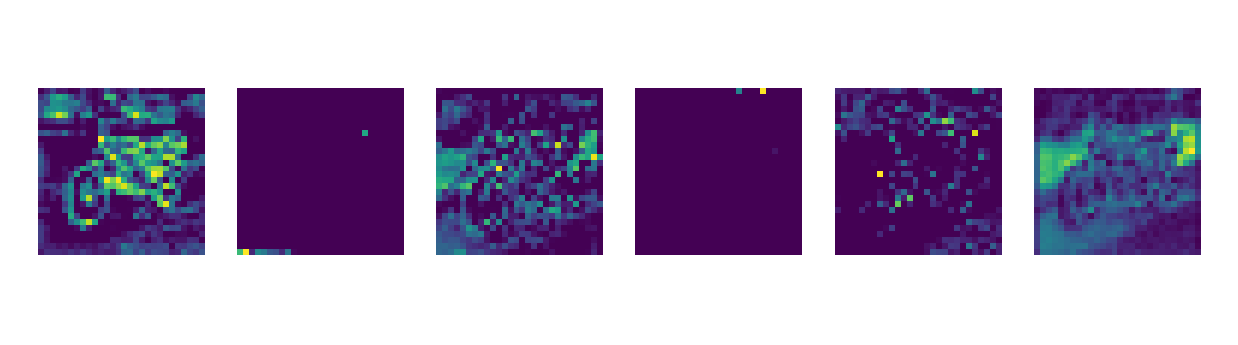
\includegraphics[width=0.8\linewidth]{V2_s_activations.png}
	\caption{CORnet-S模型V2层激活图}
	\label{f.v2_s_act}
\end{figure}

\begin{figure}[hbt]
	\centering
	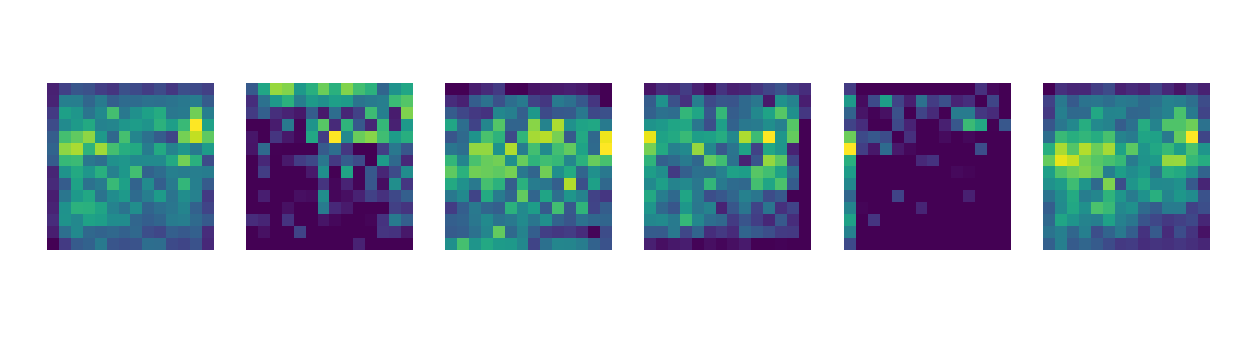
\includegraphics[width=0.8\linewidth]{V4_s_activations.png}
	\caption{CORnet-S模型V4层激活图}
	\label{f.v4_s_act}
\end{figure}

从图\ref{f.v1_s_act}(V1 层)可见,激活图主要集中在边缘与纹理区域,表现V1为对图像整体结构的低级响应,体现了模型底层的感知特性。图\ref{f.v2_s_act}(V2 层)中,响应区域虽仍零散,但开始聚焦于目标内部轮廓区域,初步展现出类别相关的空间感知。图\ref{f.v4_s_act}(V4 层)显示出更集中的激活分布,尤其在图像的中部主体区域有明显增强,说明模型已完成对部分中层语义信息的整合V。而图\ref{f.it_s_act}(IT 层)则呈现出较清晰的判别区域,激活图高度集中在摩托车的关键结构上,如前灯、车轮等,具有较强的目标识别倾向。

尽管整体趋势符合生物视觉系统的层级响应特征,但部分激活图仍存在注意力漂移现象,如V2层的部分通道对背景产生强响应。这可能反映出当前模型在缺乏显式注意机制的条件下,其选择性聚焦能力存在一定偏移,尤其在目标边界模糊、遮挡或图像背景复杂的场景下。

综上所述,Grad-CAM可视化结果表明,CORnet-S模型具有基本的空间关注能力和层级特征提取结构,但在判别区域的集中性与鲁棒性方面仍有改进空间。后续章节将尝试引入通道注意力机制,进一步优化模型对关键区域的响应特性。

